% handovers and research around it
Robot-human handovers is a process that involves a lot parameters. Object grasping, timing of social cues and head gaze are just a few of many. Identifying such parameters and their importance for a successful handover has been well researched in the past. Some studies suggest that humans prefer a minimum jerk, human-like motion when being handed over an object (\parencite{Huber2008} \parencite{Huber2008a}), therefor other research has focused on observing humans as to make robots immitate a human motion. \textcite{Chan2015} conducted a user study of handovers under different conditions and found that natural handovers may differ from reciever-oriented handovers, meaning that robots would need to take this into account when learning from demonstration to make sure it puts the human interests in priority. \textcite{Moon2014} found that only by imitating human gaze cues during a handover the robot can help the human reach for the object sooner, even before the robot finishes the movement. In the work of \textcite{Huang2015} expirements were performed as to measure adaptation between humans in collaborative tasks, concluding that adaptevily coordinating actions can increase performance in tasks such as handovers. Although \textcite{Koene2014} measured through expirements the different levels of importance between spatial and temporal precision, finding that a fast motion from the robot was better recieved from the human side than a spatially accurate end position of the robotic grasp, \textcite{Admoni2014} found through their expirements that introducing some deliberate delays in the handover help the reciever with focusing on the robot's head (i.e. gaze) and understand better it's suggestions which is suggested in \parencite{Moon2014}. \textcite{Gharbi2015} conducted handover expirements between humans and human-robot to identify preferred gaze cues during a handover. Correct grasping of objects for handovers has sometimes been connected to the type of object and it's affordances (\parencite{Song2015}, \parencite{Chan2014}) where by associating an object with different ways of manipulating it we identify a grip which is best suited when handing it over, as to increase productivity for the reciever. \textcite{Aleotti2012} developed a model based on user comfort for the reciever, in which the robot scans then environment and in a three dimensional reconstructed environment calculates the optimal handover by finding the best orientation of the object towards the human.

\begin{figure}
	\centering
	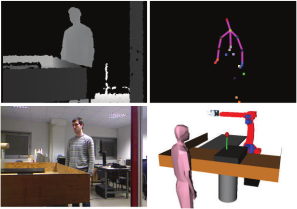
\includegraphics[width=0.5\textwidth]{img/related-work/planning-simulation.png}
	\caption{Human detection phase and handover planning in simulated environment in \parencite{Aleotti2012}}
\end{figure}

% grasping
A very important feature as to insure the success of a robot-human handover, is the grasping of objects. Robotic grasping is itself a widely researched topic and several models have been proposed to compute proper grasping of objects. Some examples of previous work that attempt at defining the representation of the object for the task of grasping include \textcite{Miller2003} who decompose an object into primitive shapes to identify good grasping points, while \textcite{Huebner2008} use a Minimum Volume Bounding Box solution to do the same. \textcite{Morales} represent objects by nine different high level descriptors of data and developed a learning framework upon this. Just as with handovers, in the domain of grasping several studies have been conducted as to observe human grasping as to make robots immitate them. \parencite{Cutkosky1990} \parencite{Feix2009} \parencite{Kang1993} made taxonomies for different grasp choices used by humans depending on objects and tasks but seeing how force closures are usually quite limited in terms of mobility (at least relative to the humand hand), this thesis will not concentrate on the actual grasping and just leave it as future work after the correct grasping region has been identified as shown in figure \ref{fig:grasp-representation}. Please refer to the work in \parencite{Sahbani2012} for a complete review of the possibilities for robotic grasping.

\begin{figure}
	\centering
	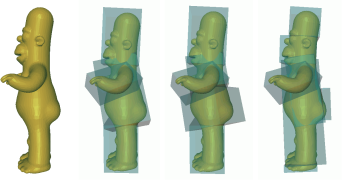
\includegraphics[width=0.7\textwidth]{img/related-work/mvbb.png}
	\caption{Minimum Volume Bounding Box on Homer model.}
\end{figure}

\begin{figure}
	\centering
	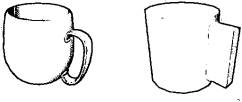
\includegraphics[width=0.3\textwidth]{img/related-work/shape-primitives.png}
	\caption{A mug model and its primitive representation.}
\end{figure}

\begin{figure}
	\centering
	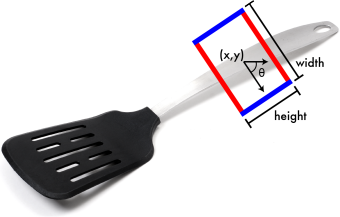
\includegraphics[width=0.3\textwidth]{img/related-work/grasp-representation.png}
	\caption{A five-dimensional grasp representation with terms of location, size and orientation. The blue lines demark the size and orientation of the gripper plates. The red lines show the approximate distance between the plates before the grasp is executed. \label{fig:grasp-representation}}
\end{figure}

% new objects
One of the challenges of robotic grasping is the ability to do grasping of objects that the robot has never seen before, nor been trained for. Some previous research do enable grasping of foreign objects, but requires a lot of data which itself needs to be labeled. For example the proposed model by \textcite{Chan2014} requires data on different ways to manipulate an object before the robot can calculate a way of grasping it and handing it over, making it hard to deploy in a new environment. Also \textcite{Huebner2008a} in a continuation of their work in \parencite{Huebner2008}, train a neural network that can be used for grasping of novel objects, but requires the network to be trained on a previously manually labeled dataset of grasps. Common within robot simulation is that data required for processing is represented by 3D models of the objects (\parencite{Miller2003}) which are not trivial to come by for newly encountered objects in a live environment as it would require the robot to see it from all angles. \textcite{Saxena2008} use several images of an object from different angles, typically obtained through stereo camera, to identify grasping sites, no longer requiring a complete 3D model of the object in question. The training of the model does however require labeled 3D models. Complete and accurate 3D models are unfortunately not always available and not feasible in an environment where a robot should learn from observing humans. Kinect sensors have become popular within robotics today because of their relatively low cost and support for depth data which can help in creating three dimensional renderings of images. \parencite{Lenz2015} \parencite{Redmon2014} \parencite{Jiang2011} propose methods for training and identifying grasp sites using RGBD from a Kinect sensor.

% learning from demonstration
The works in \parencite{Aleotti2012} \parencite{Suay2015} \parencite{Kim2004} all report good results for handovers between robots and humans, but are based on human created algorithms. An issue with human created algorithms is their limit of adaption to a wider spectrum of scenarios than those thought of when created, they can also become error prone because of human error. Machine trained models are therefor becoming more and more frequently used because they require less human intervention as well as it has become increasingly easy to collect and represent data in a more versatile way. The works of \parencite{Redmon2014} \parencite{Lenz2015} \parencite{Jiang2011} \textcite{Huebner2008a} use the advantages of machine learned models but their datasets require the time consuming task of manually labeling to train upon. However a less explored research field is to teach robots grasping and handovers by demonstrations and observations. Having robots learn by observing humans would enable faster collection of data, save time from manually labeling and allow the robot to use more human-like motions. Accuracy of sensors, correctness of the data (i.e observation, was it as good handover?) are some of the limitations of learning from observations which makes it a challenging method. The previously mentioned work in \parencite{Chan2014} collected data by observing humans interacting with objects, but as we mentioned the data covered other object interaction scenarios than a handover. \textcite{Strabala2013} trained a model using decision trees from recorded data of humans performing handovers, but they had to manually label the recorded material with eye-gaze, two-dimensional position of participants, object locations and handover positions. In other work, \textcite{Chan2015a} propose a framework for robots to learn handovers and grasp sites through demonstration. By handing objects to a robot they then have the robot repeat the handover in reverse order back to the human. They however do not have the robot learn any object features as to associate the handover to it to be used on previously untrained objects.

\begin{figure}
	\centering
	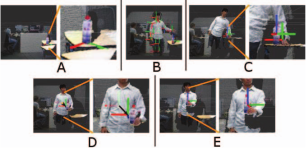
\includegraphics[width=0.5\textwidth]{img/related-work/demonstrations.png}
	\caption{Stages of extracting grasp configurations from handover demonstrations. A - Object detection. B - Human detection and tracking. C - Grasp point detection. D - Direction of torso-to-hand vector for handover cue detection. E - Object orientation at handover.}
\end{figure}

% how to use this related work for this thesis
\textcite{Redmon2014} show very promising results with their implementation, illustrating the high performance of convolutional neural networks. The problem is that the data that it needs for training is manually annoted to recognize grasp sites on objects. The framework proposed in \parencite{Chan2015a} is a good starting point for the collection of data as to train a model that can be later used for grasping and handovers. This thesis will try and combine their work by implementing a framework for collecting data through demonstration from humans and process it as to train a convolutional neural network that can later identify grasping sites on novel objects by RGBD images.

\begin{figure}
	\centering
	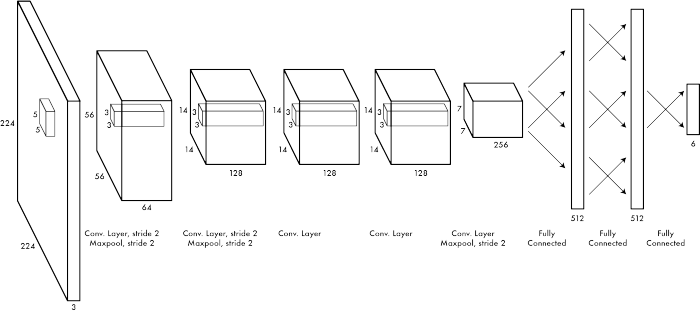
\includegraphics[width=\textwidth]{img/related-work/cnn-architecture.png}
	\caption{Full architecture used in \parencite{Redmon2014}}
\end{figure}

